\documentclass[10pt,a4paper]{article}
\usepackage[margin=17mm]{geometry}
\usepackage{amsmath,amssymb,booktabs,graphicx,hyperref}
\hypersetup{colorlinks=true,urlcolor=blue,linkcolor=blue}
\setlength{\parindent}{0pt}\setlength{\parskip}{5pt}
\newcommand{\pageheading}[1]{{\Large\bfseries #1}\par\vspace{3mm}}
\begin{document}
\pageheading{Smoothing Frank--Wolfe: convex schedule comparison}
\textbf{4 November 2026.} Small synthetic CPU benchmark with a certified convex reference.

\textbf{Scope.} This is a schedule and prefactor comparison within one shared stochastic momentum--Moreau smoothing--Frank--Wolfe update. The problem is convex. It supplies an implementation check and a schedule ablation; it does not demonstrate an algorithmic advantage or the contribution of the nonconvex analysis.

Let $\Omega$ contain $N=1000$ observed entries of a $50\times50$ matrix $Y$. We solve
\[
\min_{X\in C} f(X)+g(TX),\qquad
f(X)=\frac1{2N}\sum_{(i,j)\in\Omega}(X_{ij}-Y_{ij})^2,
\]
\[
C=\{X:\|X\|_*\le40\},\qquad g=\iota_D,\quad
D=[-1,1]^{50\times50},\quad T=I.
\]
The nuclear norm is the sum of singular values. The linear minimization oracle is $-40uv^\top$, where $(u,v)$ is a leading singular-vector pair of the search direction. This experiment uses a full SVD to evaluate that oracle accurately. The projection onto $D$ clips every entry to $[-1,1]$.

\textbf{Stochastic oracle.} Draw $(i,j)$ uniformly from $\Omega$ and return
\[
Q(X;i,j)=(X_{ij}-Y_{ij})e_ie_j^\top,\qquad
\mathbb E[Q(X;i,j)\mid X]=\nabla f(X).
\]
A batch averages $q$ independent draws with replacement. Repeated indices are accumulated. The finite-sum objective is globally smooth; $C$ is compact and convex; $D$ is closed and convex; zero lies in the interior of both sets. Component gradients have uniformly bounded variance on $C$. Thus the stochastic oracle and geometry meet the stated problem assumptions. Convexity makes this a special case of the manuscript's nonconvex setting.

\textbf{Data and reference.} A fixed seed, 20261104, generates a rank-five signal scaled to maximum absolute entry 0.8, plus Gaussian noise with standard deviation 0.6. Exactly 40\% of entries are observed; every row and column has observations. The other 1500 entries are excluded from optimization. Some noisy observations exceed the fitted-value box. Radius 20 made the box inactive at the independently solved optimum; the documented pre-campaign design check selected radius 40, the first proposed candidate with both constraints active. No optimizer comparison informed that choice.

The independently evaluated primal/dual reference bracket is
\[
0.061233455500\ \le f^\star\le\ 0.061233455778,
\qquad U-L=2.78\times10^{-10}.
\]
The feasible primal point supplies $U$. With CVXPY box multiplier $Z$, the lower bound is computed independently as
\[
L=f(X_r)-\langle\nabla f(X_r),X_r\rangle
-40\|\nabla f(X_r)+Z\|_{\mathrm{op}}-\|Z\|_1.
\]
This is a floating-point convex certificate, not interval arithmetic. Both the nuclear bound and two box entries are active. Initial loss at zero is 0.191074531.

\textbf{Meaning of the plotted loss.} Each raw iterate stays in $C$. For reporting only, form $\widehat X=X/\max(1,\max_{ij}|X_{ij}|)$, which also lies in $D$. This radial repair never feeds back into the optimizer. The true feasible objective error lies in $[f(\widehat X)-U,f(\widehat X)-L]$; plots use its upper endpoint. Raw loss and box violation are saved separately.

\newpage
\pageheading{Fresh-seed performance under different schedules}
For zero-based update $k\ge0$, SFRAMES uses
\[
\gamma_k=\gamma_0(k+1)^{-3/4},\quad
\rho_k=\rho_0(k+1)^{-1/2},\quad
\beta_k=\beta_0(k+1)^{-1/4}.
\]
Its momentum starts at the first sampled smooth gradient. SHCGM uses the published Algorithm 1 schedules, written with the same zero-based index:
\[
\gamma_k=\frac9{k+9},\quad \rho_k=\frac4{(k+8)^{2/3}},\quad
\beta_k=\frac{\beta_0}{\sqrt{k+9}}.
\]
Both use the same momentum, Moreau-penalty gradient, LMO and convex-combination update. SHCGM starts from zero momentum with first weight one, so its first estimate is also the first sampled gradient. The schedules and prefactors distinguish the tested configurations. No line search is used.

\begin{center}\small
\begin{tabular}{lrrr}\toprule
Selected configuration & $\gamma_0$ & $\rho_0$ & $\beta_0$\\\midrule
SFRAMES tuned & 0.3 & 0.3 & 100 \\
SHCGM & fixed & fixed & 1000 \\
SFRAMES unit & 1 & 1 & 100 \\
\bottomrule\end{tabular}
\end{center}
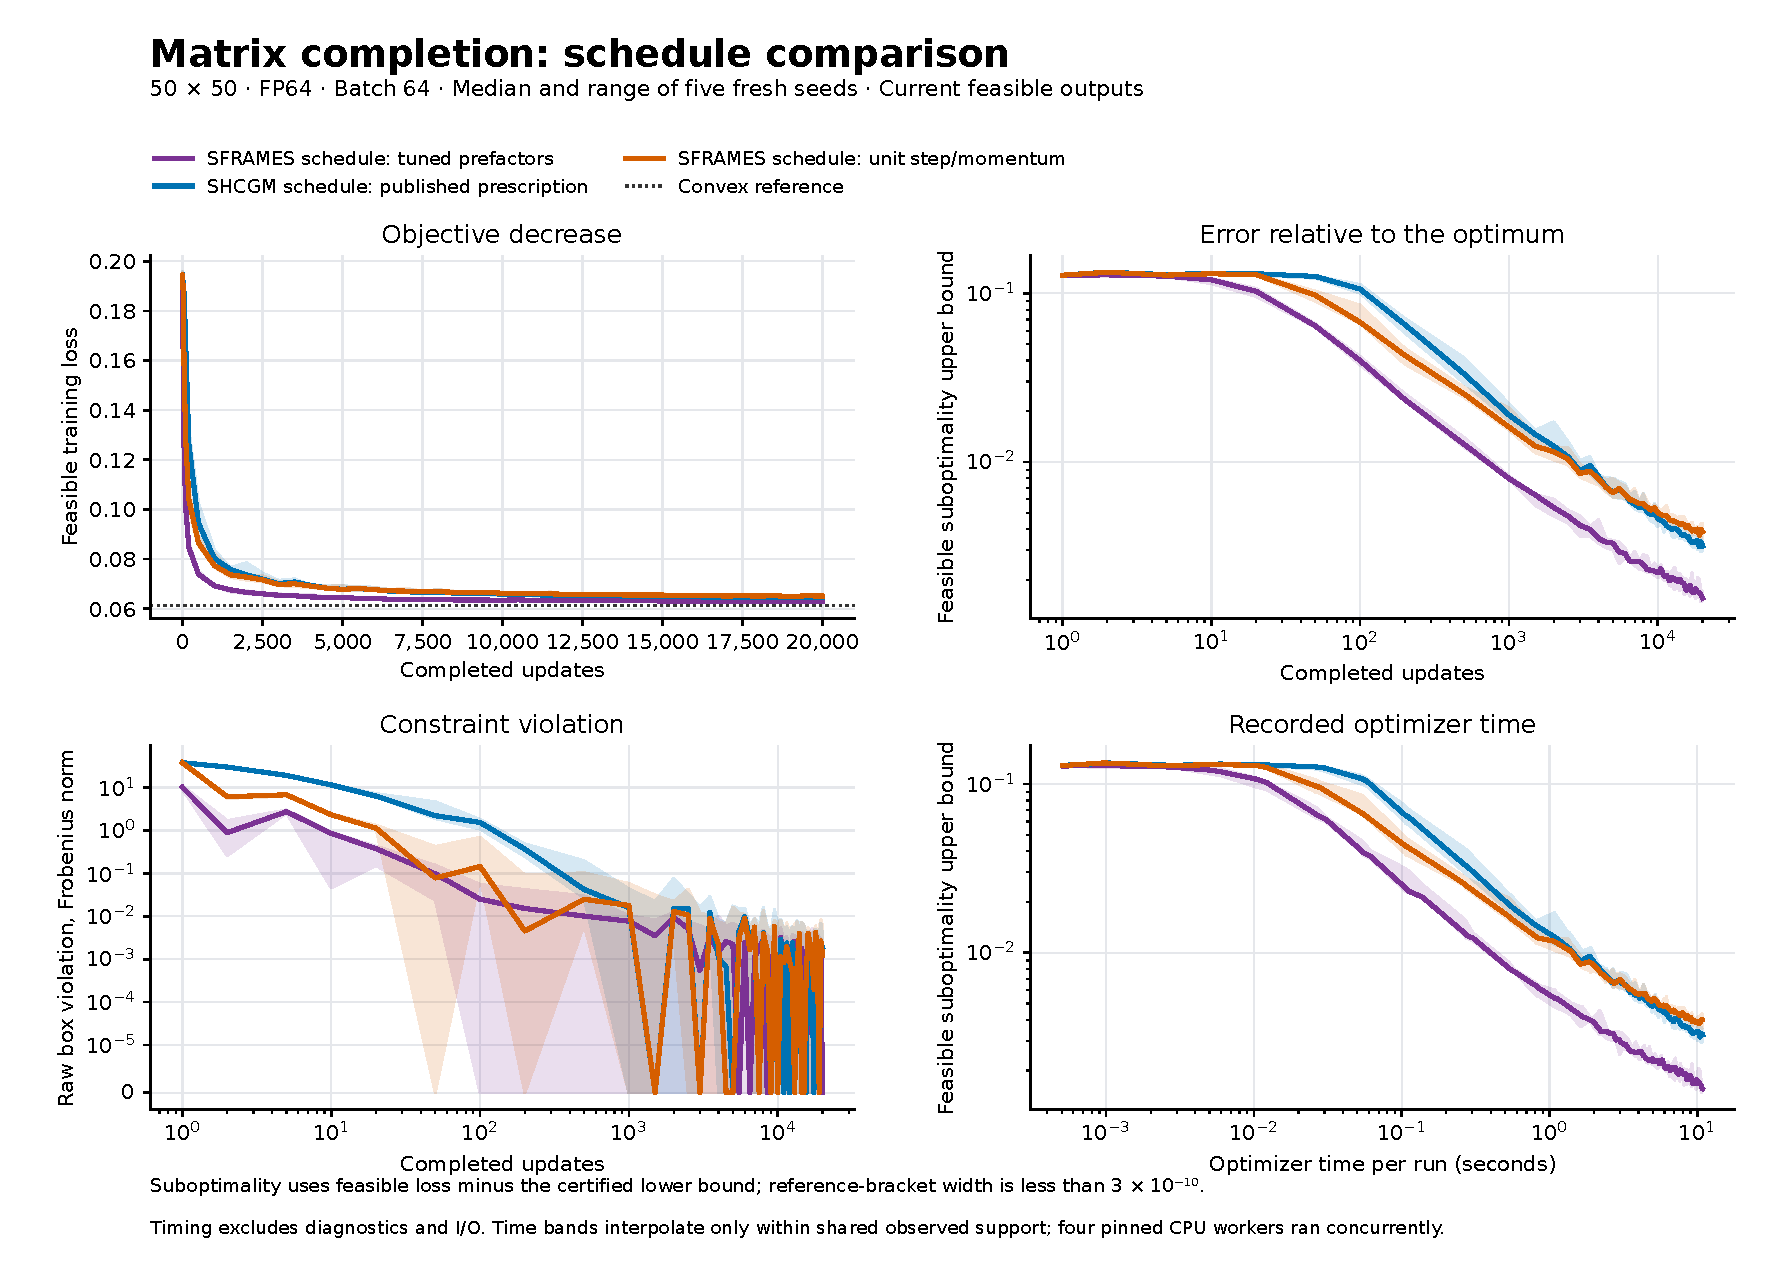
\includegraphics[width=\linewidth]{comparison_batch64.pdf}
\vspace{-3mm}
\begin{center}\small
\begin{tabular}{lrrr}\toprule
Batch64; five fresh seeds & Median feasible loss & Seed range & Initial gap closed\\\midrule
SFRAMES tuned & 0.062787 & [0.062748, 0.062925] & 98.8\% \\
SHCGM & 0.064408 & [0.064233, 0.064578] & 97.6\% \\
SFRAMES unit & 0.065097 & [0.064772, 0.065568] & 97.0\% \\
\bottomrule\end{tabular}
\end{center}
The unit-prefactor SFRAMES control fixes both step and momentum prefactors to one; only its smoothing prefactor is selected. Its five fresh seeds are shared with the other configurations.

\newpage
\pageheading{Sample budgets, parameter selection, and timing}
Each method receives 16 candidate configurations, two development seeds (101,102), batch 64, and 20000 updates per run. SFRAMES searches $\gamma_0,\rho_0\in\{0.3,1\}$ and $\beta_0/N\in\{0.1,1,10,100\}$. SHCGM keeps its published step/momentum schedules and searches 16 logarithmically spaced values of $\beta_0/N$ from0.01 to1000. Each method selects the lowest median final feasible training loss. The unit-prefactor SFRAMES control selects among its four smoothing values. The selected SFRAMES step, momentum and smoothing prefactors lie at the lower tested grid boundaries; this is the best tested configuration in a fixed grid, not evidence that tuning is globally optimal. The grid was not expanded after observing confirmation results.

Five fresh seeds (201--205) confirm each selection. The same selected parameters are reused at batches 16, 64, 256; these batches are not retuned. For each seed and batch, all methods receive identical random index streams. Their sampled gradients differ because their iterates differ. Each run uses FP64, starts from zero, and completes 20000 updates.

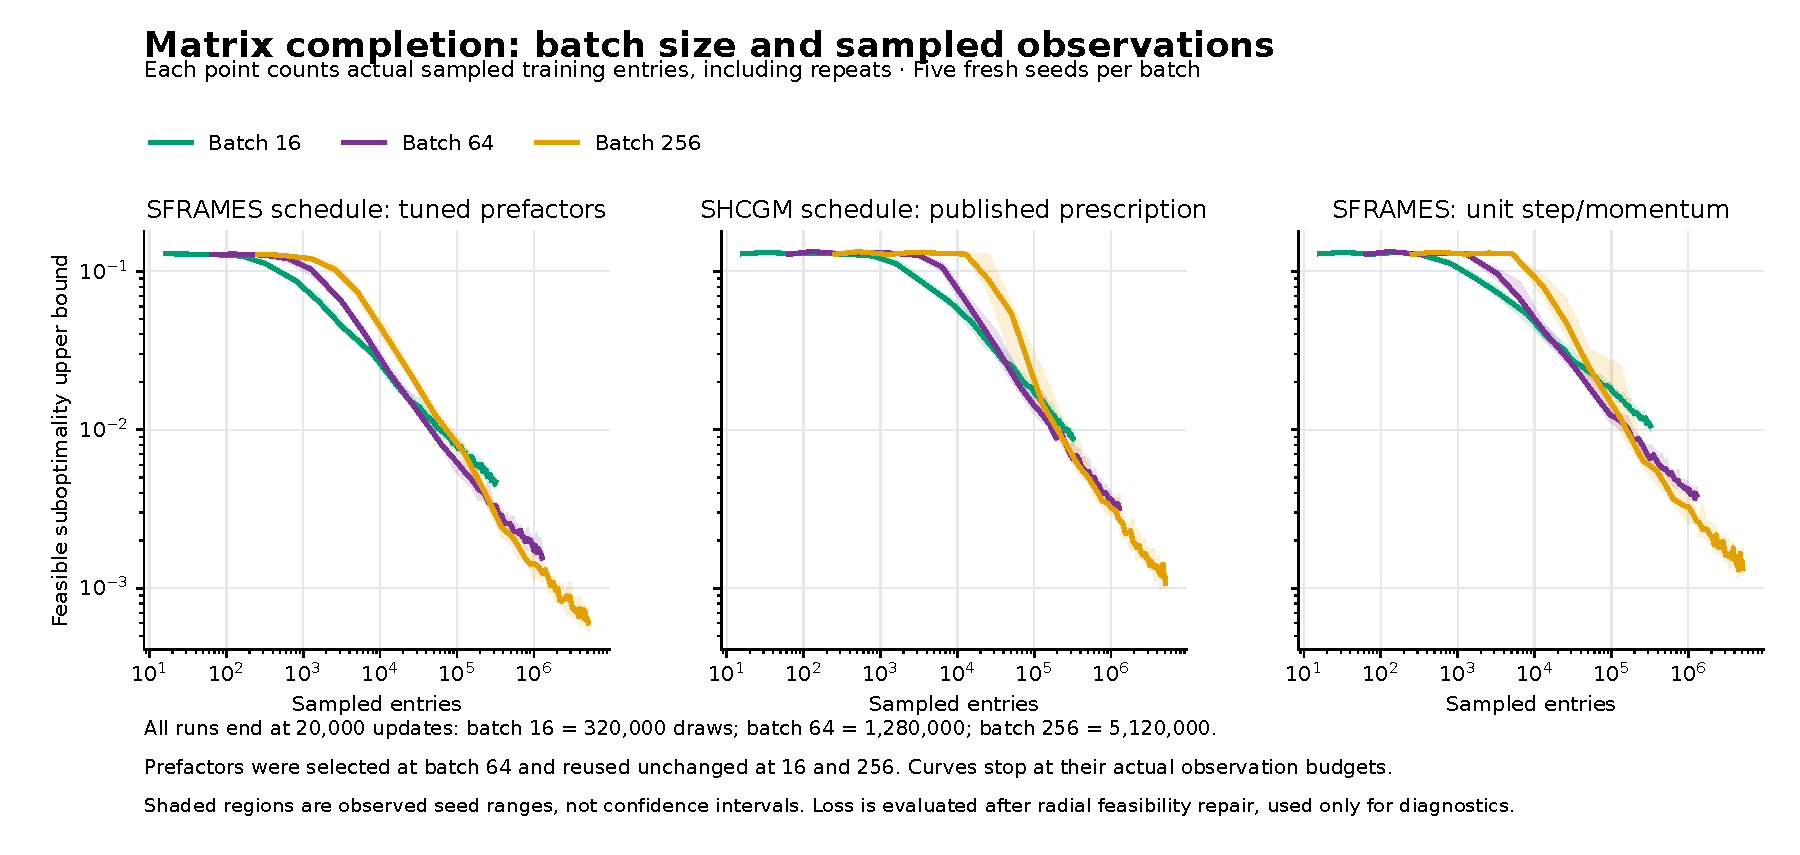
\includegraphics[width=\linewidth]{batch_sample_comparison.pdf}

\begin{center}\small
\begin{tabular}{lrrrrr}\toprule
Method & Batch & Gap upper bound & Box violation & Optimizer(s) & Diagnostics(s)\\\midrule
SFRAMES tuned & 16 & 0.004695 & 0.000216 & 10.75 & 4.19 \\
SFRAMES tuned & 64 & 0.001554 & 0 & 10.95 & 4.23 \\
SFRAMES tuned & 256 & 0.0006039 & 0 & 11.15 & 4.25 \\
SHCGM & 16 & 0.008792 & 0 & 10.79 & 4.21 \\
SHCGM & 64 & 0.003174 & 0.00189 & 10.95 & 4.25 \\
SHCGM & 256 & 0.001074 & 0 & 11.15 & 4.28 \\
SFRAMES unit & 16 & 0.01061 & 0 & 10.82 & 4.22 \\
SFRAMES unit & 64 & 0.003863 & 0.00124 & 10.88 & 4.22 \\
SFRAMES unit & 256 & 0.001328 & 0 & 11.08 & 4.27 \\
\bottomrule\end{tabular}
\end{center}
Table entries are medians across five fresh seeds at the final update. The gap is evaluated at the feasible diagnostic output; box violation is evaluated at the raw iterate.

\textbf{Timing.} Four processes run concurrently on four pinned physical cores of an AMD Ryzen 5 PRO 3400G, one numerical-library thread per process. Optimizer timing includes sampling, momentum, penalty gradient, the full-SVD LMO, and the update. Exact-gap diagnostics, objective/feasibility evaluations, feasible repair, and file output are excluded. Diagnostic time is recorded separately. Time curves interpolate only within the common observed time support across seeds and do not extrapolate endpoints. Concurrent CPU measurements do not provide uncontended latency estimates, and tuning cost is excluded from per-run curves.

\textbf{Interpretation.} At batch 64, the SFRAMES tuned schedule has the lowest median final feasible loss in this finite grid. Both named prescriptions instantiate the same update family on this convex problem. The observed difference concerns schedules and constants, not a distinct algorithmic mechanism. SHCGM uses convexity in its schedule analysis; these finite-horizon results do not overturn that theory. SFRAMES also received more kinds of tunable constants (step, momentum and smoothing, versus smoothing alone), despite equal candidate counts. This experiment cannot support a claim of algorithmic superiority or demonstrate the value of the nonconvex extension.

\newpage
\pageheading{The theorem statistic and the existing nonconvex example}
For the new experiment, let $H_k=\nabla f(X_k)+(X_k-\operatorname{clip}(X_k))/\beta_k$. The exact smoothed Frank--Wolfe gap is
\[
G_k=\langle H_k,X_k\rangle+40\|H_k\|_{\mathrm{op}}.
\]
The reported theorem statistic is $K^{-1}\sum_{k=0}^{K-1}G_k$, computed at \emph{every} pre-update iterate, then averaged across seeds. It is neither a sparse-checkpoint average nor a gap computed from the noisy momentum estimator. The SFRAMES unit-prefactor control follows the displayed manuscript prescription; its smoothing prefactor remains positive and tuned. The expected averaged gap has the stated $O(K^{-1/4})$ guarantee. These finite runs illustrate behavior and cannot establish an asymptotic rate.

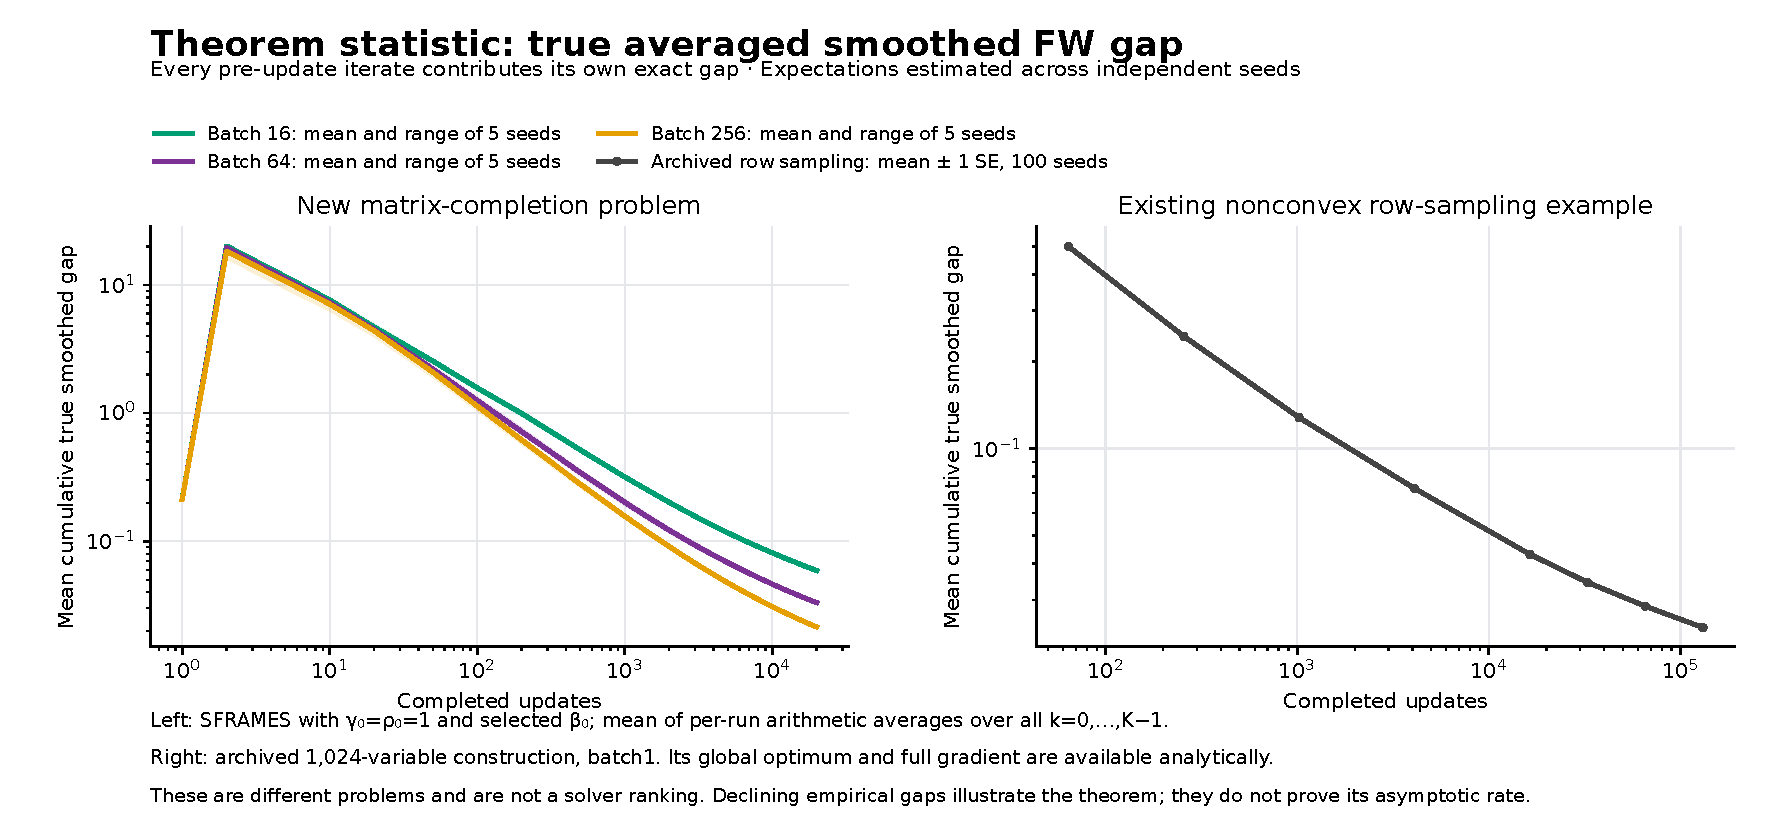
\includegraphics[width=\linewidth]{theorem_statistic.pdf}

\textbf{Reused experiment, not rerun.} The archived 1024-variable problem is
\[
\min_{\|x\|_1\le1}\ \|Ax-b\|^2-\frac58(u^\top x)^2+\iota_{\mathbb R_+^{1024}}(x),\qquad A^\top A=I/2.
\]
It uses genuine independent uniform row sampling, batch 1, 100 seeds, and 131072 updates. Its true averaged smoothed gap decreases from 0.127887 at 1024 updates to 0.024035 at 131072. Its global optimum is $13/256=0.05078125$, while the final feasible loss has median 0.05838535, leaving median objective gap 0.007604. Thus the stationarity trend does not imply near-optimal objective values. The orthogonal synthetic design also makes the full gradient cheap; it is a theorem illustration, not practical efficiency evidence. Original artifacts are preserved; the original gap plot is copied beside this report.

\textbf{Sources and reproducibility.} SHCGM: Locatello, Yurtsever, Fercoq and Cevher, \href{https://proceedings.neurips.cc/paper/2019/file/bf40d1cbb2ba9fdad19821fc140fa50c-Paper.pdf}{Stochastic Frank--Wolfe for Composite Convex Minimization}, NeurIPS 2019, Algorithm 1 and Section 4.3. The present normalized synthetic problem uses that algorithm, but does not claim the published MovieLens objective values. SFRAMES: supplied \texttt{Nonsmooth\_FW-7.pdf}, Corollary 2.10 and Proposition 2.11. The implementation follows the positive Moreau-penalty gradient from its definition; the draft's opposite sign in Algorithm 1 is recorded in the audit.

Run configurations, selected parameters, data/source checksums, reference duals, complete diagnostic curves, optimizer and diagnostic timing, and validation receipts accompany this report. See \texttt{summary.json}, \texttt{curves.csv}, \texttt{endpoints.csv}, \texttt{campaign\_config.json}, \texttt{selection.json}, and \texttt{provenance/} in the experiment directory. Historical source: \texttt{/home/tony/frames\_stochastic\_rows\_1024\_20261014}.
\end{document}
